\documentclass{article}
\usepackage[utf8]{inputenc}
\usepackage[spanish]{babel}
\usepackage{listings}
\usepackage{graphicx}
\usepackage{chicago}
\graphicspath{ {images/} }
\usepackage{cite}

\begin{document}

\begin{titlepage}
    \begin{center}
        \vspace*{1cm}
            
        \huge
        \textbf{Taller Memorias}
            
        \vspace{1.5cm}
        \LARGE
        Informática II
            
        \vspace{1.5cm}
            
        \textbf{Jorge Sebastian Arroyo Estrada}
            
        \vfill
            
        \vspace{0.8cm}
            
        \Large
        Despartamento de Ingeniería Electrónica y Telecomunicaciones\\
        Universidad de Antioquia\\
        Medellín\\
        Septiembre de 2020
            
    \end{center}
\end{titlepage}

\tableofcontents

\section{La memoria de un computador}
“Memoria” en un computador, es un término genérico usado para referirse a las partes de la computadora donde toda la información y programas son almacenados y trabajados por los microprocesadores para generar los resultados que los usuarios requieran.\newline
Desde el primer momento en que se enciende el computador hasta el momento en que se apaga, el microprocesador hace uso constante de la memoria. Existen varios tipos de memoria en los computadores con diferentes capacidades, velocidades y funciones. La memoria en una computadora es vital, ya que, sin esta, la computadora no encendería.\cite{ref}

\section{Tipos de memoria en una computadora}
La memoria es uno de los componentes fundamentales para el correcto funcionamiento de una computadora, ya que su existencia permite que la computadora puede arrancar, se procesen los datos, se ejecuten las instrucciones para los distintos programas y demás.\newline
No obstante, una computadora trabaja con cuatro tipos de memorias diferentes, que sirven para realizar diversas funciones. Estas son la memoria RAM, la memoria ROM, la memoria SRAM o Caché y la memoria Virtual.\newline

\textbf{Memoria RAM:}
La Random Access Memory o memoria RAM es la más importante, sin ella la computadora se vería imposibilitada para funcionar correctamente. Se emplea para almacenar temporalmente las instrucciones o los datos. Este tipo de memoria informática también se le conoce como memoria de escritura y lectura porque pueden leerse o escribirse los datos en ella. Desde algunos procesos temporales, tales como las modificaciones en los archivos, hasta todas aquellas instrucciones que hacen posible que se ejecuten las aplicaciones que tenemos instaladas en nuestro ordenador, se guardan en la RAM.\newline
Se caracteriza por tener un acceso aleatorio para la lectura y escritura de datos, mientras mayor sea su capacidad de almacenamiento, mayor será su respuesta en cuanto a rendimiento de la computadora.\newline

Figura demostrativa de la memoria RAM (\ref{fig_ram})\newline

\begin{figure}[h]
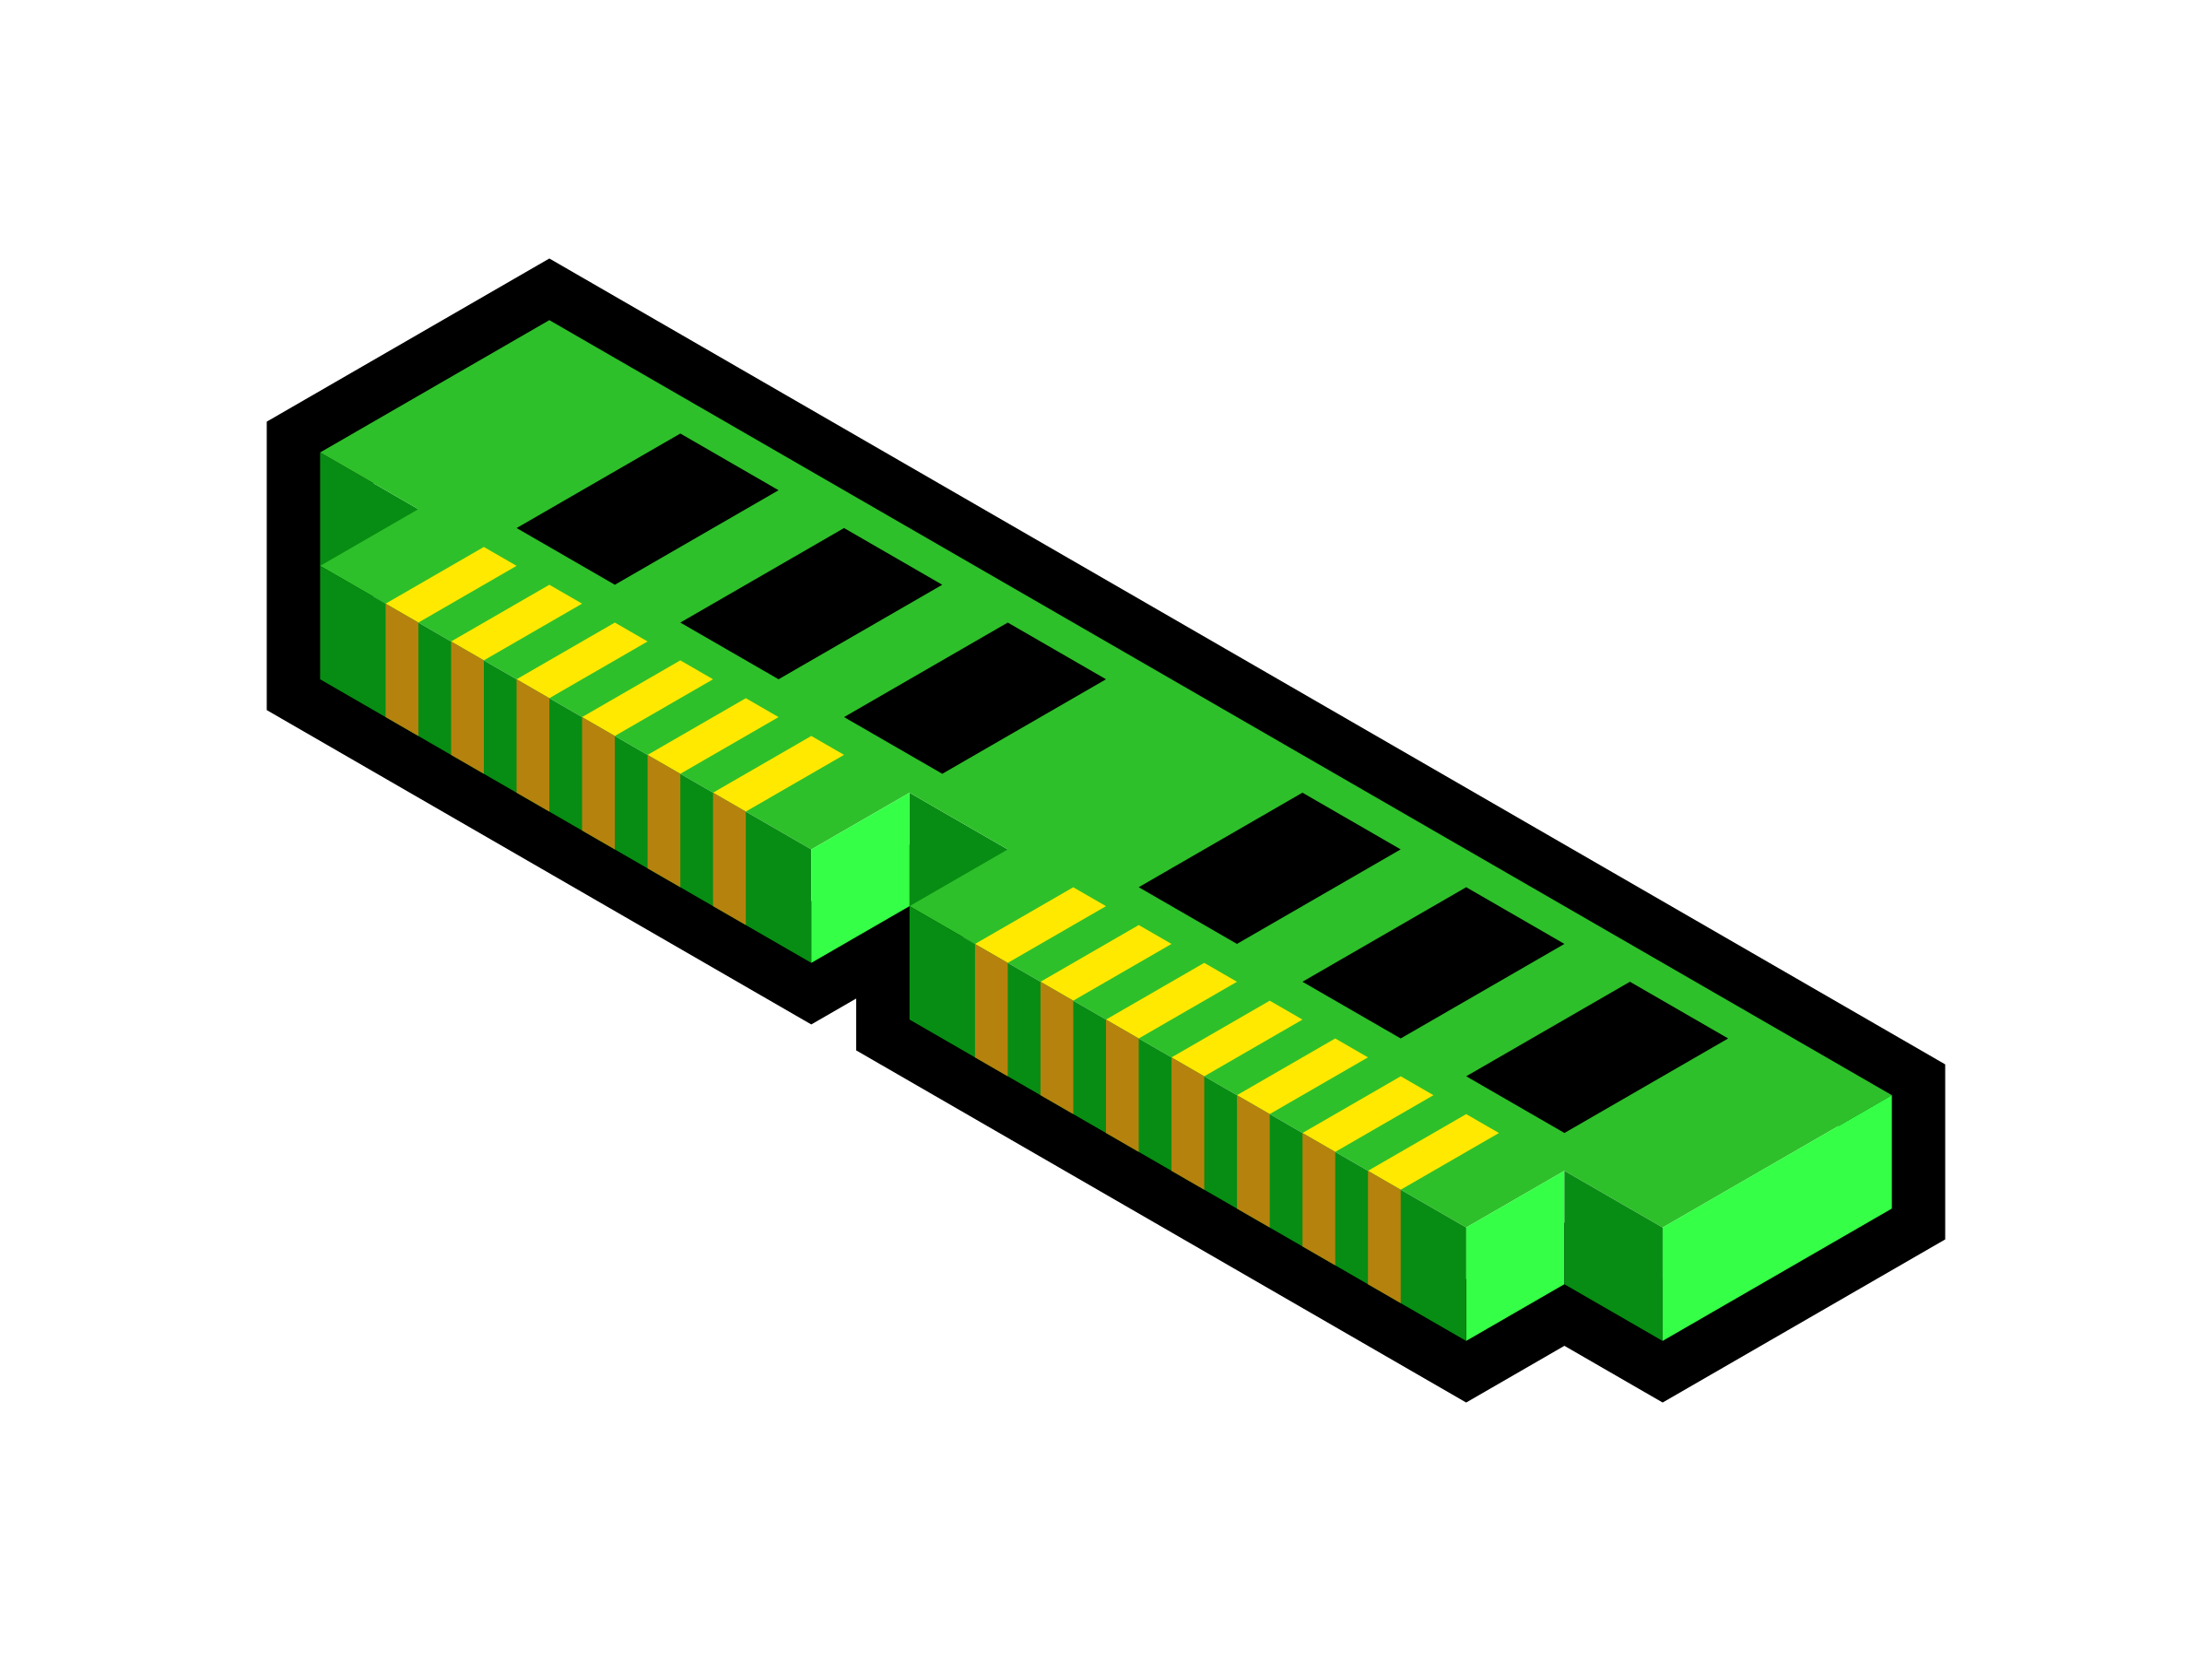
\includegraphics[width=5cm]{ram.png}
\centering
\caption{RAM}
\label{fig_ram}
\end{figure}

\textbf{Memoria ROM:}
La memoria ROM o Read Only Memory (Memoria de sólo lectura), es básicamente, un chip en el que se puede almacenar en su interior toda la información necesaria para que los dispositivos electrónicos, bien sean computadoras o un teléfono inteligente dé inicio a su proceso de arranque. Se caracteriza por ser una memoria de tipo secuencial, ya que se deben recorrer todos los datos hasta que se logre ubicar la información que se necesita. Tiene como principal función la de tener toda la capacidad para conservar los datos que contiene, aun cuando no exista una fuente de energía que la alimente, aspecto muy opuesto al de las memorias RAM, que, si requieren estar energizadas, porque de no ser así las mismas pierden inmediatamente su contenido.\newline
La memoria ROM la podemos encontrar incorporada a la motherboard o placa madre, esta es empleada por la computadora para que pueda producirse el inicio de la BIOS o Basic Input/Output System, que es un programa que contiene todas las instrucciones precisas para poder guiar correctamente a la computadora durante el arranque.\newline

Figura demostrativa de la memoria ROM (\ref{fig_rom})\newline

\begin{figure}[h]
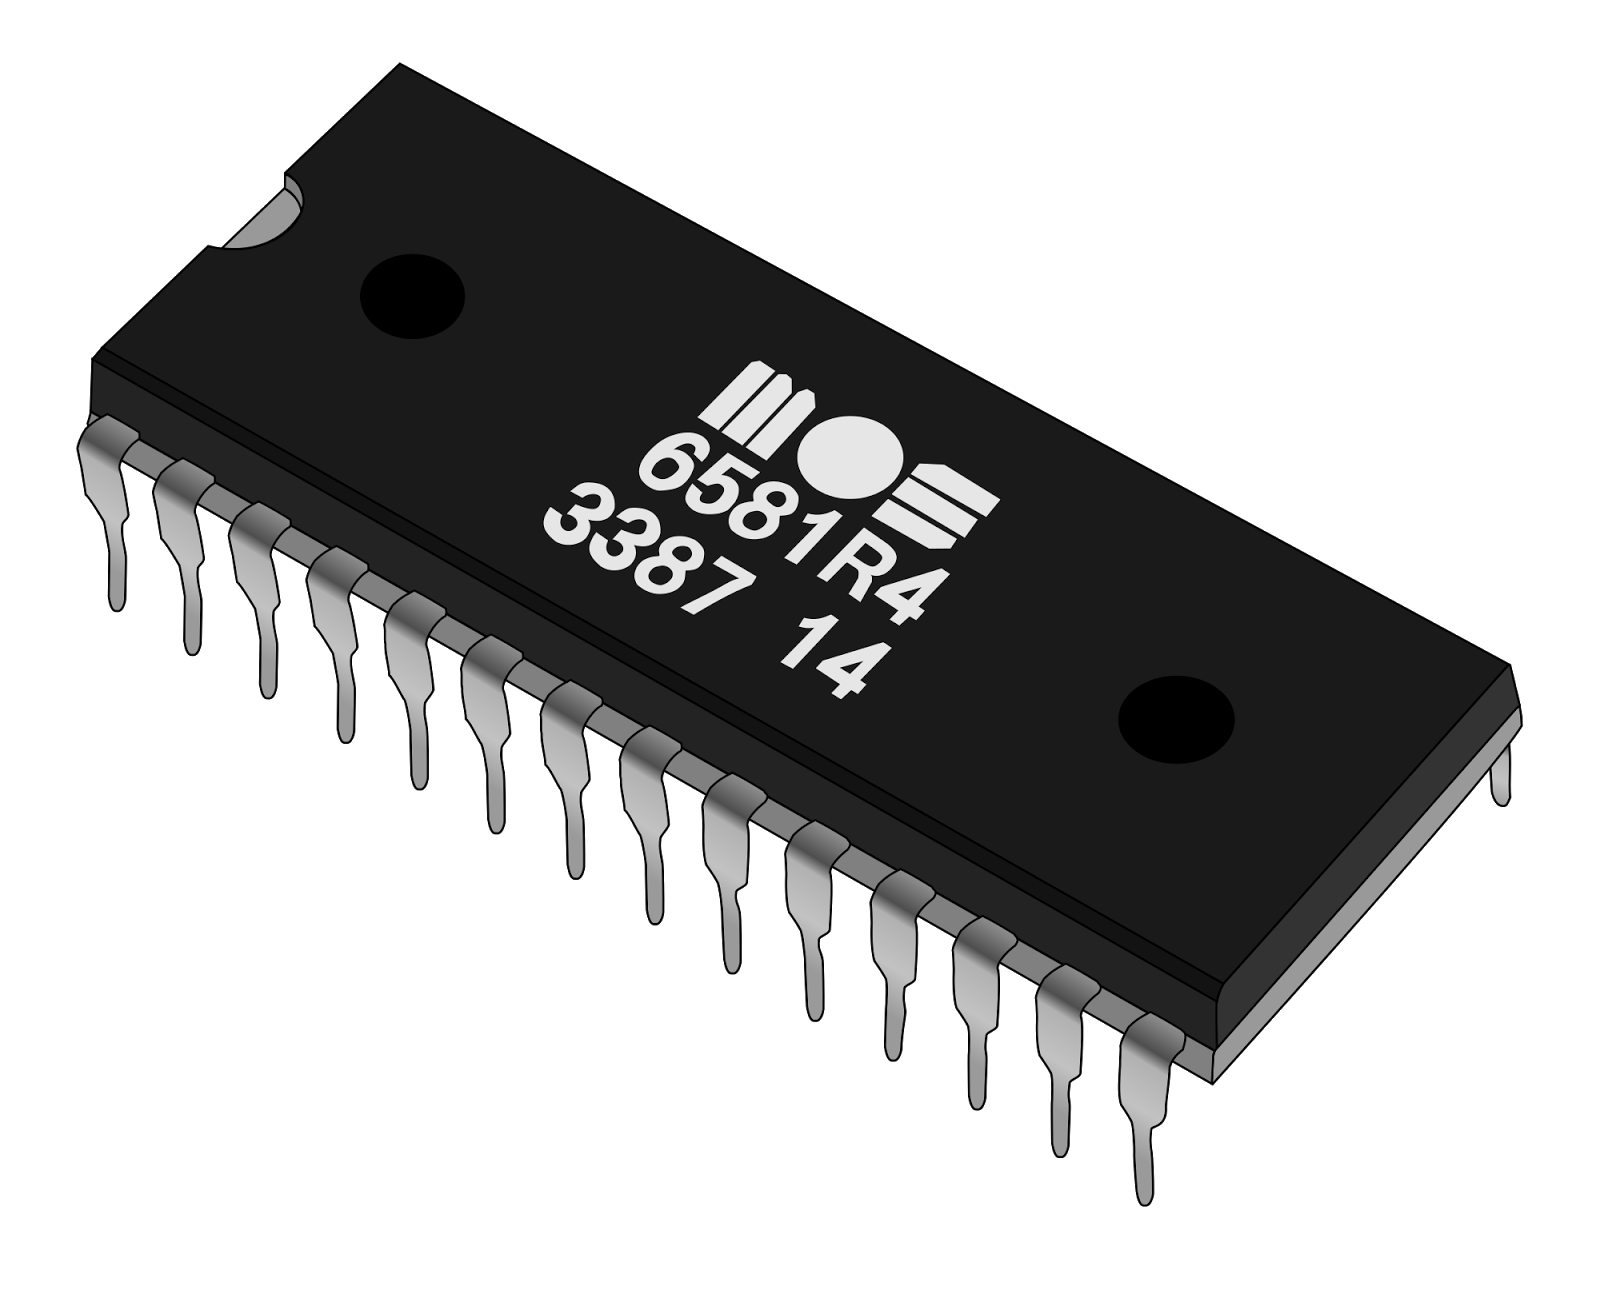
\includegraphics[width=5cm]{rom.png}
\centering
\caption{RAM}
\label{fig_rom}
\end{figure}

\textbf{Memoria Caché:}
Es uno de los recursos más valiosos con los que cuenta una CPU o Central Processing Unit (Unidad Central de Procesamiento), la cual se utiliza para almacenar de manera temporalmente todos los datos que fueron procesados recientemente en un búfer especial o la memoria auxiliar.\newline
Esta memoria trabaja de manera muy similar a la memoria principal del CPU, pero lo hace con mayor velocidad a pesar de que su tamaño es mucho menor. Dada su eficacia es capaz de proveer al microprocesador de un tiempo extra para que acceda a los datos que son utilizados con mayor frecuencia, sin necesidad de tener que rastrear en su lugar de origen cada vez que sea necesario.\newline
Es así como esta memoria alterna se coloca entre el CPU y la memoria RAM y es capaz de proveer del empuje necesario adicional en tiempo y ahorro de recursos al sistema.\newline

Figura demostrativa de la memoria caché (\ref{fig_cache})\newline

\begin{figure}[h]
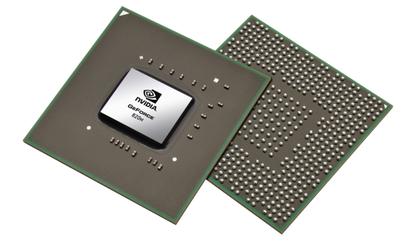
\includegraphics[width=5cm]{cache.png}
\centering
\caption{Caché}
\label{fig_cache}
\end{figure}

\textbf{Memoria virtual:}
Este tipo de memorias informáticas las podemos encontrar en computadoras cuyo sistema operativo sea Microsoft Windows o Linux. Son muy similares a la caché, pero fueron diseñadas para ser usada exclusivamente por el sistema operativo. En el sistema operativo Linux se encuentra ubicada en una partición distinta del disco, mientras que, por el contrario, en el sistema operativo de Windows, esta es un archivo que está en el interior del sistema operativo.\newline
A través de este método, el sistema operativo puede disponer de mayor capacidad de memoria de la que la que ya tiene disponible. Y en ocasiones muchas de las aplicaciones, requieren de acceso a muchos más datos que los que pueden ser almacenados en una memoria física, por tal razón es que se recurre a la memoria virtual.\cite{Google}\newpage

Figura demostrativa de la jerarquia de las memorias (\ref{fig_mem})\newline

\begin{figure}[h]
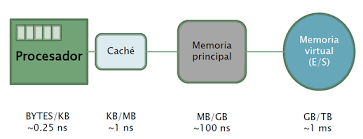
\includegraphics[width=8cm]{virtual.png}
\centering
\caption{Jerarquia de memorias}
\label{fig_mem}
\end{figure}

\section{¿Cómo se gestiona la memoria en un computador?}
\textbf{Gestión de memoria:}
La administración de memoria se refiere a los distintos métodos y operaciones que se encargan de obtener la máxima utilidad de la memoria, organizando los procesos y programas que se ejecutan de tal forma que se aproveche de la mejor manera posible el espacio disponible.\newline
Para poder lograrlo, la operación principal que realiza es trasladar la información que deberá ser ejecutada por la unidad central de procesamiento o procesador, a la memoria principal. Actualmente, esta administración se conoce como memoria virtual, porque no es la memoria física del procesador sino una memoria virtual que la representa. Entre algunas ventajas, esta memoria permite que el sistema cuente con una memoria más extensa teniendo la misma memoria real, por lo que esta se puede utilizar de manera más eficiente. Y por supuesto, que los programas que son utilizados no ocupen lugar innecesario.\newline

\Large\textbf{Características}\newline

\normalsize\textbf{Protección:}
La protección de memoria es un método para controlar el uso de memoria en una computadora, y es parte esencial de prácticamente todos los sistemas operativos modernos. El principal propósito de la protección de memoria es evitar que un proceso en un sistema operativo acceda a la memoria que no le ha sido asignada.\newline

\textbf{Memoria compartida:}
Aunque la memoria utilizada por diferentes procesos suele estar protegida, algunos procesos puede que sí tengan que compartir información y, para ello, han de acceder la misma sección de memoria. La memoria compartida es una de las técnicas más rápidas para posibilitar la comunicación entre procesos.\newline

\textbf{Organización lógica:}
Permiten que los programas se escriban como módulos compilables y ejecutables por separado.\newline

\textbf{Organización física:}
La memoria suele dividirse en un almacenamiento primario de alta velocidad y uno secundario de menor velocidad.  La gestión de memoria del sistema operativo se ocupa de trasladar la información entre estos dos niveles de memoria.\newline

\textbf{¿Por qué se necesita la gestión de memoria?}\newline

Para optimizar el espacio y poder cargar o intercambiar los programas que van hacer ejecutados del disco duro a la memoria principal.\newline
El administrador de memoria se encarga de llevar un registro de las partes de la memoria que están en uso y de las que no. Si detecta que hay una parte que ya no está en uso, la libera para poder asignarla a los procesos que la necesiten.
El administrador de memoria proporciona protección y uso compartido, es decir, facilitar un espacio de memoria para cada proceso y controlar que ninguno de ellos trabaje en zonas de memoria que no le han sido asignados.\newline
Administrar el intercambio entre la memoria principal y el disco en los casos en los que la memoria principal no le pueda dar capacidad a todos los procesos que tienen necesidad de ella.\cite{Sistemas}

\section{¿Qué hace que una memoria sea más rápida que otra? ¿Por qué esto es importante?}

En un computador hay varios tipos de memoria, ordenados en jerarquías de velocidad y capacidad. Memoria Cache L1, L2 y L3, Memoria RAM, Memoria Virtual, Disco Duro Cuanto más bajamos en la lista desde la memoria Cache hacia el disco duro, decrece la velocidad de los distintos tipos de memoria y aumenta su capacidad.

\bibliographystyle{IEEEtran}
\bibliography{references}

\end{document}
